\documentclass[11pt]{scrartcl} 
%%%%%%%%%%%%%%%%%%%%%%%%%%%%%%%%%%%%%%%%%%%%%%%%%%%%%%%%%%%%%%%%%%%%

%\usepackage{graphics}
\usepackage{float}
\usepackage{subfigure}
\usepackage{graphicx}
\usepackage{amssymb}
\usepackage{amsmath}
\usepackage{amsfonts}
\usepackage{amssymb}
\usepackage{amstext}
\usepackage{amsbsy}
\usepackage{xspace}
\usepackage{verbatim}
\usepackage{csvsimple}
\usepackage{sectsty}
\usepackage{tikz}

%%%%%%%%%%%%%%%%%%%%%%%%%%%%%%%%%%%%%%%%%%%%%%%%%%%%%%%%%%%%%%%%%%%%
% operators
\renewcommand{\div}{\vec{\nabla}\! \cdot \!}
\newcommand{\grad}{\vec{\nabla}}
% latex shortcuts
\newcommand{\bea}{\begin{eqnarray}}
\newcommand{\eea}{\end{eqnarray}}
\newcommand{\be}{\begin{equation}}
\newcommand{\ee}{\end{equation}}
\newcommand{\bal}{\begin{align}}
\newcommand{\eali}{\end{align}}
\newcommand{\bi}{\begin{itemize}}
\newcommand{\ei}{\end{itemize}}
\newcommand{\ben}{\begin{enumerate}}
\newcommand{\een}{\end{enumerate}}
% DGFEM commands
\newcommand{\jmp}[1]{[\![#1]\!]}                     % jump
\newcommand{\mvl}[1]{\{\!\!\{#1\}\!\!\}}             % mean value
\newcommand{\kef}{\ensuremath{k_{\textit{eff}}}}
%\newcommand{\keff}{{\text{k}$_\textit{eff}$}\xspace}
\newcommand{\keff}{\kef\xspace}
% shortcut for domain notation
%\newcommand{\D}{\mathcal{D}}
% vector shortcuts
\newcommand{\vo}{\vec{\Omega}}
\newcommand{\vr}{\vec{r}}
\newcommand{\vn}{\vec{n}}
\newcommand{\vnk}{\vec{\mathbf{n}}}
\newcommand{\vj}{\vec{J}}
% extra space
\newcommand{\qq}{\quad\quad}
% common reference commands
\newcommand{\eqt}[1]{Eq.~(\ref{#1})}                     % equation
\newcommand{\fig}[1]{Fig.~\ref{#1}}                      % figure
\newcommand{\tbl}[1]{Table~\ref{#1}}                     % table

\newcommand{\ud}{\,\mathrm{d}}
\newcommand{\mt}[1]{\marginpar{\tiny #1}}
\newcommand{\D}{\ensuremath{\mathcal{D}}}
\allowdisplaybreaks

\newcommand{\subj}{\\\hspace{-5mm}\textbf{Subject: IQS with multiple PRKE Parameter Updates within Macro Steps}}
\newcommand{\from}{\vspace{-20mm}\hspace{-1mm} \normalfont From: Zachary Prince \\}
\newcommand{\toms}{\hspace{-5mm} To: Jean Ragusa and Yaqi Wang \\}
\newcommand{\datet}{\hspace{-5mm} Date: \today \\}

\allsectionsfont{\centering \large}
\setlength\parindent{0pt}
\usepackage{ccaption}
\setlength{\abovecaptionskip}{0mm} %lowers the distance of captions to the figure
\setlength{\oddsidemargin}{0in}
\setlength{\evensidemargin}{1in}
\setlength{\textwidth}{6.5in}

% tikz stuff
\usetikzlibrary{shapes,arrows,positioning}
\pgfdeclarelayer{background}
\pgfdeclarelayer{foreground}
\pgfsetlayers{background,main,foreground}
\tikzstyle{greenblock}=[rectangle, rounded corners, draw, align=center, top color=white, bottom color=green!20, ultra thick, minimum width=60mm, minimum height=15mm,]
\tikzstyle{blueblock}=[rectangle, rounded corners, draw, align=center, top color=white, bottom color=blue!20, ultra thick, minimum width=60mm, minimum height=15mm]
\tikzstyle{reddiamond}=[diamond, draw, align=center, top color=white, bottom color=red!20, ultra thick, minimum width=60mm, aspect=2]
\newcommand{\tikzback}[5]{
 \begin{pgfonlayer}{background}
  \path (#1.west |- #2.north)+(-0.5,0.75) node (a1) {};
  \path (#3.east |- #4.south)+(+0.5,-0.25) node (a2) {};
  \path[fill=yellow!10,rounded corners, draw=black!100, dashed] (a1) rectangle (a2);
   \path (#3.east |- #2.north)+(0,1.25)--(#1.west |- #2.north) node[midway] (#5-n) {};
   \path (#3.east |- #2.south)+(0,-0.35)--(#1.west |- #2.south) node[midway] (#5-s) {};
   \path (#1.west |- #2.north)+(-0.75,0)--(#1.west |- #4.south) node[midway] (#5-w) {};
 \end{pgfonlayer}}

%%%%%%%%%%%%%%%%%%%%%%%%%%%%%%%%%%%%%%%%%%%%%%%%%%%%%%%%%%%%%%%%%%%%%
%
%   BEGIN DOCUMENT
%
%%%%%%%%%%%%%%%%%%%%%%%%%%%%%%%%%%%%%%%%%%%%%%%%%%%%%%%%%%%%%%%%%%%%%
\begin{document}
%%%%%%%%%%%%%%%%%%%%%%%%%%%%%%%%%%%%%%%%%%%%%%%%%%%%%%%%%%%%%%%%%%%%%

%%---------------------------------------------------------------------------%%
%% OPTIONS FOR NOTE
%%---------------------------------------------------------------------------%%
\title{\normalfont \Large TEXAS A\&M UNIVERSITY}
\subtitle{\normalfont Dwight Look College of Engineering \\ Department of Nuclear Engineering \\ \Large \textbf{Research Memo}}
\date{}

%%---------------------------------------------------------------------------%%
%% BEGIN NOTE
%%---------------------------------------------------------------------------%%

\maketitle
\from
\toms
\datet
\subj

%%---------------------------------------------------------------------------%%
\section{\large Initial Implementation of Multiple PRKE Parameter Updates}
%%---------------------------------------------------------------------------%%

The purpose of this note is to describe how IQS updates the PRKE parameters within macro time steps and the results of the initial implementation.  The impetus of this initiative was the underwhelming results from applying IQS to the LRA benchmark.  It is strongly believed that the treatment of the coupling between temperature and the PRKE parameters were to blame for results.  Figure~\ref{fig:lra_bad} shows that IQS only improves the time step size by less than half at $t=1.44$ s.  This is the point where the power is at a max, so the temperatue is changing rapidly, but the shape is not changing significantly.  Figure~\ref{fig:lra_good} shows the error at $t=1.40$ s, where IQS performs significantly better.  At this point, the temperature is not changing significantly.  Therefore, IQS does not treat temperature with enough accuracy to see significant improvement over brute force.

\begin{figure}[!htpb]
\centering
\subfigure[LRA convergence results at $t=1.44s$]{
\label{fig:lra_bad}
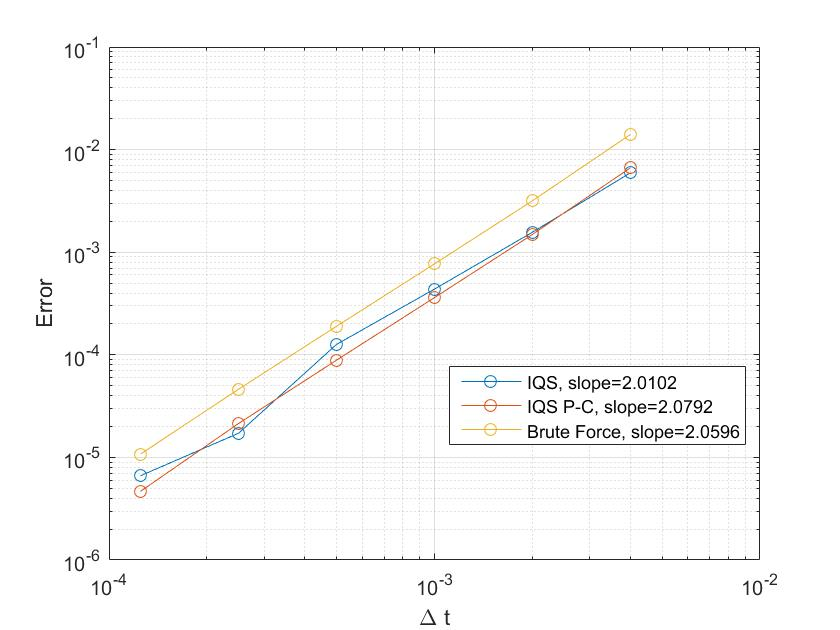
\includegraphics[width=0.52\textwidth]{mp_figs/lra_bad.jpg} }
\hspace{-15mm}
\subfigure[LRA convergence results at $t=1.40$]{
\label{fig:lra_good}
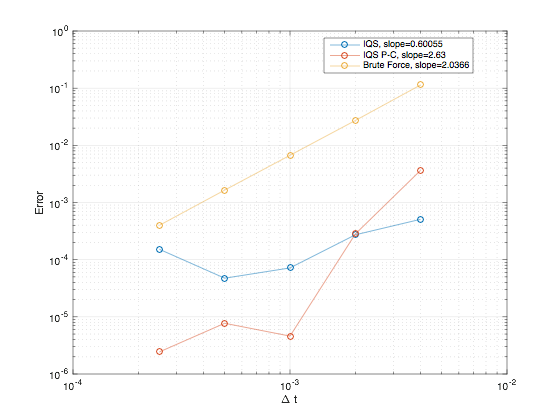
\includegraphics[width=0.52\textwidth]{mp_figs/lra_good.png} }
\caption{LRA convergence plots with only one temperature updated each macro step}
\end{figure}

Temperature has the most effect when calculating the PRKE parameters to solve for amplitude.  So in order to more accurately capture the behavior of the flux, the PRKE parameters and temperature need to be evaluated multiple times within each macro step. To visualize this process the system is setup with three different time scales, as shown in Figures~\ref{fig:time}~and~\ref{fig:timepc}.  Figures~\ref{fig:proc}~and\ref{fig:procpc} show the same processes in more detail.  The occurrence that there are three updates in the figures is arbitrary, the number of temperature updates can be set by the user.

\begin{figure}[H]
\centering
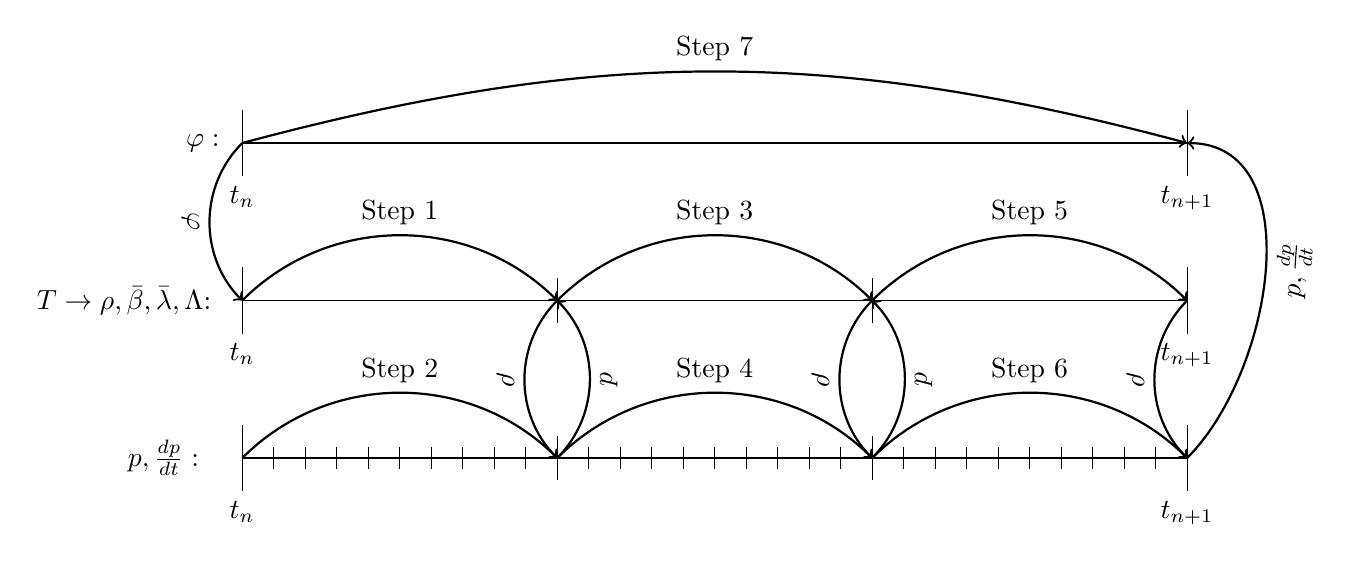
\begin{tikzpicture}[scale=2]
%Shape
\draw[] (0,2) -- (6,2) ;
\foreach \x in  {0,6}
\draw[shift={(\x,2)},color=black] (0pt,6pt) -- (0pt,-6pt);
\draw[shift={(0,2)},color=black] (0pt,0pt) -- (0pt,-6pt) node[below] {$t_n$};
\draw[shift={(6,2)},color=black] (0pt,0pt) -- (0pt,-6pt) node[below] {$t_{n+1}$};
\node(shape) at (-.25,2) {$\varphi:$};

%Temp/Params
\draw[] (0,1) -- (6,1) ;
\foreach \x in  {0,6}
\draw[shift={(\x,1)},color=black] (0pt,6pt) -- (0pt,-6pt);
\foreach \x in  {2,4}
\draw[shift={(\x,1)},color=black] (0pt,4pt) -- (0pt,-4pt);
\draw[shift={(0,1)},color=black] (0pt,0pt) -- (0pt,-6pt) node[below] {$t_n$};
\draw[shift={(6,1)},color=black] (0pt,0pt) -- (0pt,-6pt) node[below] {$t_{n+1}$};
\node(temp) at (-.75,1) {$T \rightarrow \rho, \bar{\beta}, \bar{\lambda}, \Lambda$:};

% PRKE
\draw[] (0,0) -- (6,0) ;
\foreach \x in  {0,6}
\draw[shift={(\x,0)},color=black] (0pt,6pt) -- (0pt,-6pt);
\foreach \x in  {0,2,4,6}
\draw[shift={(\x,0)},color=black] (0pt,4pt) -- (0pt,-4pt);
\foreach \x in  {0,0.2,0.4,0.6,0.8,1,1.2,1.4,1.6,1.8,2,2.2,2.4,2.6,2.8,3,3.2,3.4,3.6,3.8,4,4.2,4.4,4.6,4.8,5,5.2,5.4,5.6,5.8,6}
\draw[shift={(\x,0)},color=black] (0pt,2pt) -- (0pt,-2pt);
\draw[shift={(0,0)},color=black] (0pt,0pt) -- (0pt,-6pt) node[below] {$t_n$};
\draw[shift={(6,0)},color=black] (0pt,0pt) -- (0pt,-6pt) node[below] {$t_{n+1}$};
\node(prke) at (-.5,0) {$p, \frac{dp}{dt}:$};

\draw (0,0) edge[out=45,in=135,->,thick] node[above,sloped] {Step 2} (2,0);
\draw (2,0) edge[out=45,in=135,->,thick] node[above,sloped] {Step 4} (4,0);
\draw (4,0) edge[out=45,in=135,->,thick] node[above,sloped] {Step 6} (6,0);
\draw (0,1) edge[out=45,in=135,->,thick] node[above,sloped] {Step 1} (2,1);
\draw (2,1) edge[out=45,in=135,->,thick] node[above,sloped] {Step 3} (4,1);
\draw (4,1) edge[out=45,in=135,->,thick] node[above,sloped] {Step 5} (6,1);
\draw (0,2) edge[out=15,in=165,->,thick] node[above,sloped] {Step 7} (6,2);

\draw (0,2) edge[out=-135,in=135,->,thick] node[below,sloped] {$\varphi$} (0,1);
\draw (2,1) edge[out=-135,in=135,->,thick] node[below,sloped] {$\rho$} (2,0);
\draw (2,0) edge[out=45,in=-45,->,thick] node[below,sloped] {$p$} (2,1);
\draw (4,1) edge[out=-135,in=135,->,thick] node[below,sloped] {$\rho$} (4,0);
\draw (4,0) edge[out=45,in=-45,->,thick] node[below,sloped] {$p$} (4,1);
\draw (6,1) edge[out=-135,in=135,->,thick] node[below,sloped] {$\rho$} (6,0);
\draw (6,0) edge[out=45,in=0,->,thick] node[below,sloped] {$p, \frac{dp}{dt}$} (6,2);

\end{tikzpicture}
\caption{Time scales and process of regular IQS}
\label{fig:time}
\end{figure}

\begin{figure}[H]
\centering
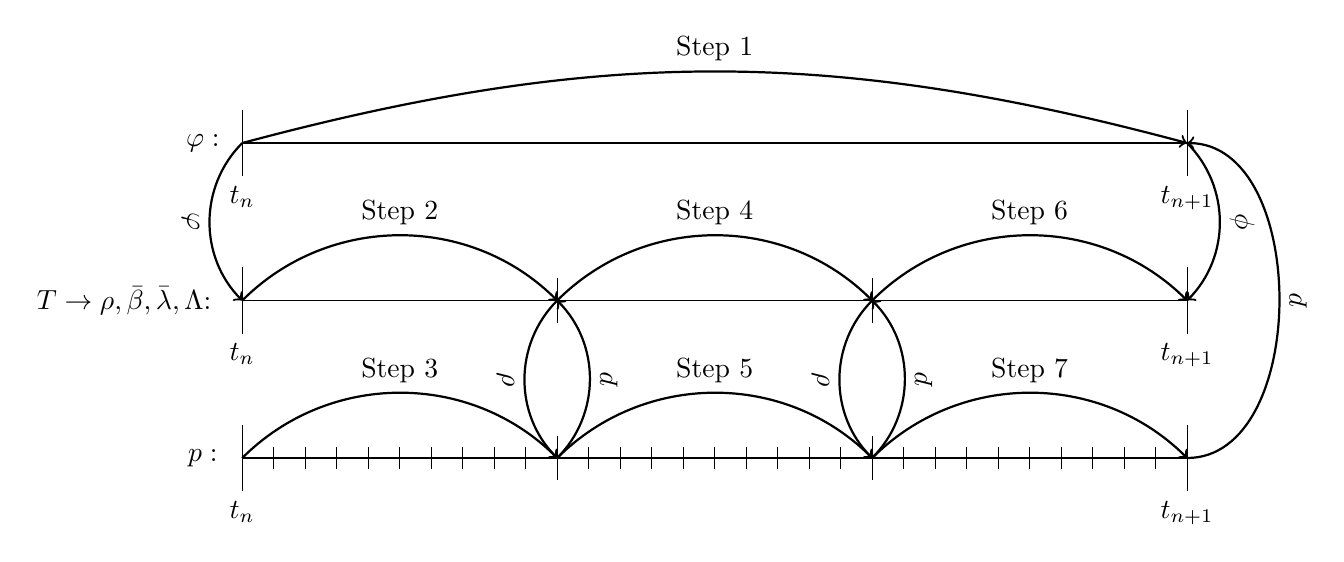
\begin{tikzpicture}[scale=2]
%Shape
\draw[] (0,2) -- (6,2) ;
\foreach \x in  {0,6}
\draw[shift={(\x,2)},color=black] (0pt,6pt) -- (0pt,-6pt);
\draw[shift={(0,2)},color=black] (0pt,0pt) -- (0pt,-6pt) node[below] {$t_n$};
\draw[shift={(6,2)},color=black] (0pt,0pt) -- (0pt,-6pt) node[below] {$t_{n+1}$};
\node(shape) at (-.25,2) {$\varphi:$};

%Temp/Params
\draw[] (0,1) -- (6,1) ;
\foreach \x in  {0,6}
\draw[shift={(\x,1)},color=black] (0pt,6pt) -- (0pt,-6pt);
\foreach \x in  {2,4}
\draw[shift={(\x,1)},color=black] (0pt,4pt) -- (0pt,-4pt);
\draw[shift={(0,1)},color=black] (0pt,0pt) -- (0pt,-6pt) node[below] {$t_n$};
\draw[shift={(6,1)},color=black] (0pt,0pt) -- (0pt,-6pt) node[below] {$t_{n+1}$};
\node(temp) at (-.75,1) {$T \rightarrow \rho, \bar{\beta}, \bar{\lambda}, \Lambda$:};

% PRKE
\draw[] (0,0) -- (6,0) ;
\foreach \x in  {0,6}
\draw[shift={(\x,0)},color=black] (0pt,6pt) -- (0pt,-6pt);
\foreach \x in  {0,2,4,6}
\draw[shift={(\x,0)},color=black] (0pt,4pt) -- (0pt,-4pt);
\foreach \x in  {0,0.2,0.4,0.6,0.8,1,1.2,1.4,1.6,1.8,2,2.2,2.4,2.6,2.8,3,3.2,3.4,3.6,3.8,4,4.2,4.4,4.6,4.8,5,5.2,5.4,5.6,5.8,6}
\draw[shift={(\x,0)},color=black] (0pt,2pt) -- (0pt,-2pt);
\draw[shift={(0,0)},color=black] (0pt,0pt) -- (0pt,-6pt) node[below] {$t_n$};
\draw[shift={(6,0)},color=black] (0pt,0pt) -- (0pt,-6pt) node[below] {$t_{n+1}$};
\node(prke) at (-.25,0) {$p:$};

\draw (0,0) edge[out=45,in=135,->,thick] node[above,sloped] {Step 3} (2,0);
\draw (2,0) edge[out=45,in=135,->,thick] node[above,sloped] {Step 5} (4,0);
\draw (4,0) edge[out=45,in=135,->,thick] node[above,sloped] {Step 7} (6,0);
\draw (0,1) edge[out=45,in=135,->,thick] node[above,sloped] {Step 2} (2,1);
\draw (2,1) edge[out=45,in=135,->,thick] node[above,sloped] {Step 4} (4,1);
\draw (4,1) edge[out=45,in=135,->,thick] node[above,sloped] {Step 6} (6,1);
\draw (0,2) edge[out=15,in=165,->,thick] node[above,sloped] {Step 1} (6,2);

\draw (0,2) edge[out=-135,in=135,->,thick] node[below,sloped] {$\varphi$} (0,1);
\draw (2,1) edge[out=-135,in=135,->,thick] node[below,sloped] {$\rho$} (2,0);
\draw (2,0) edge[out=45,in=-45,->,thick] node[below,sloped] {$p$} (2,1);
\draw (4,1) edge[out=-135,in=135,->,thick] node[below,sloped] {$\rho$} (4,0);
\draw (4,0) edge[out=45,in=-45,->,thick] node[below,sloped] {$p$} (4,1);
\draw (6,0) edge[out=0,in=0,->,thick] node[below,sloped] {$p$} (6,2);
\draw (6,2) edge[out=-45,in=45,->,thick] node[above,sloped] {$\phi$} (6,1);

\end{tikzpicture}
\caption{Time scales and process of IQS P-C}
\label{fig:timepc}
\end{figure}

\begin{figure}[!htpb]
\centering
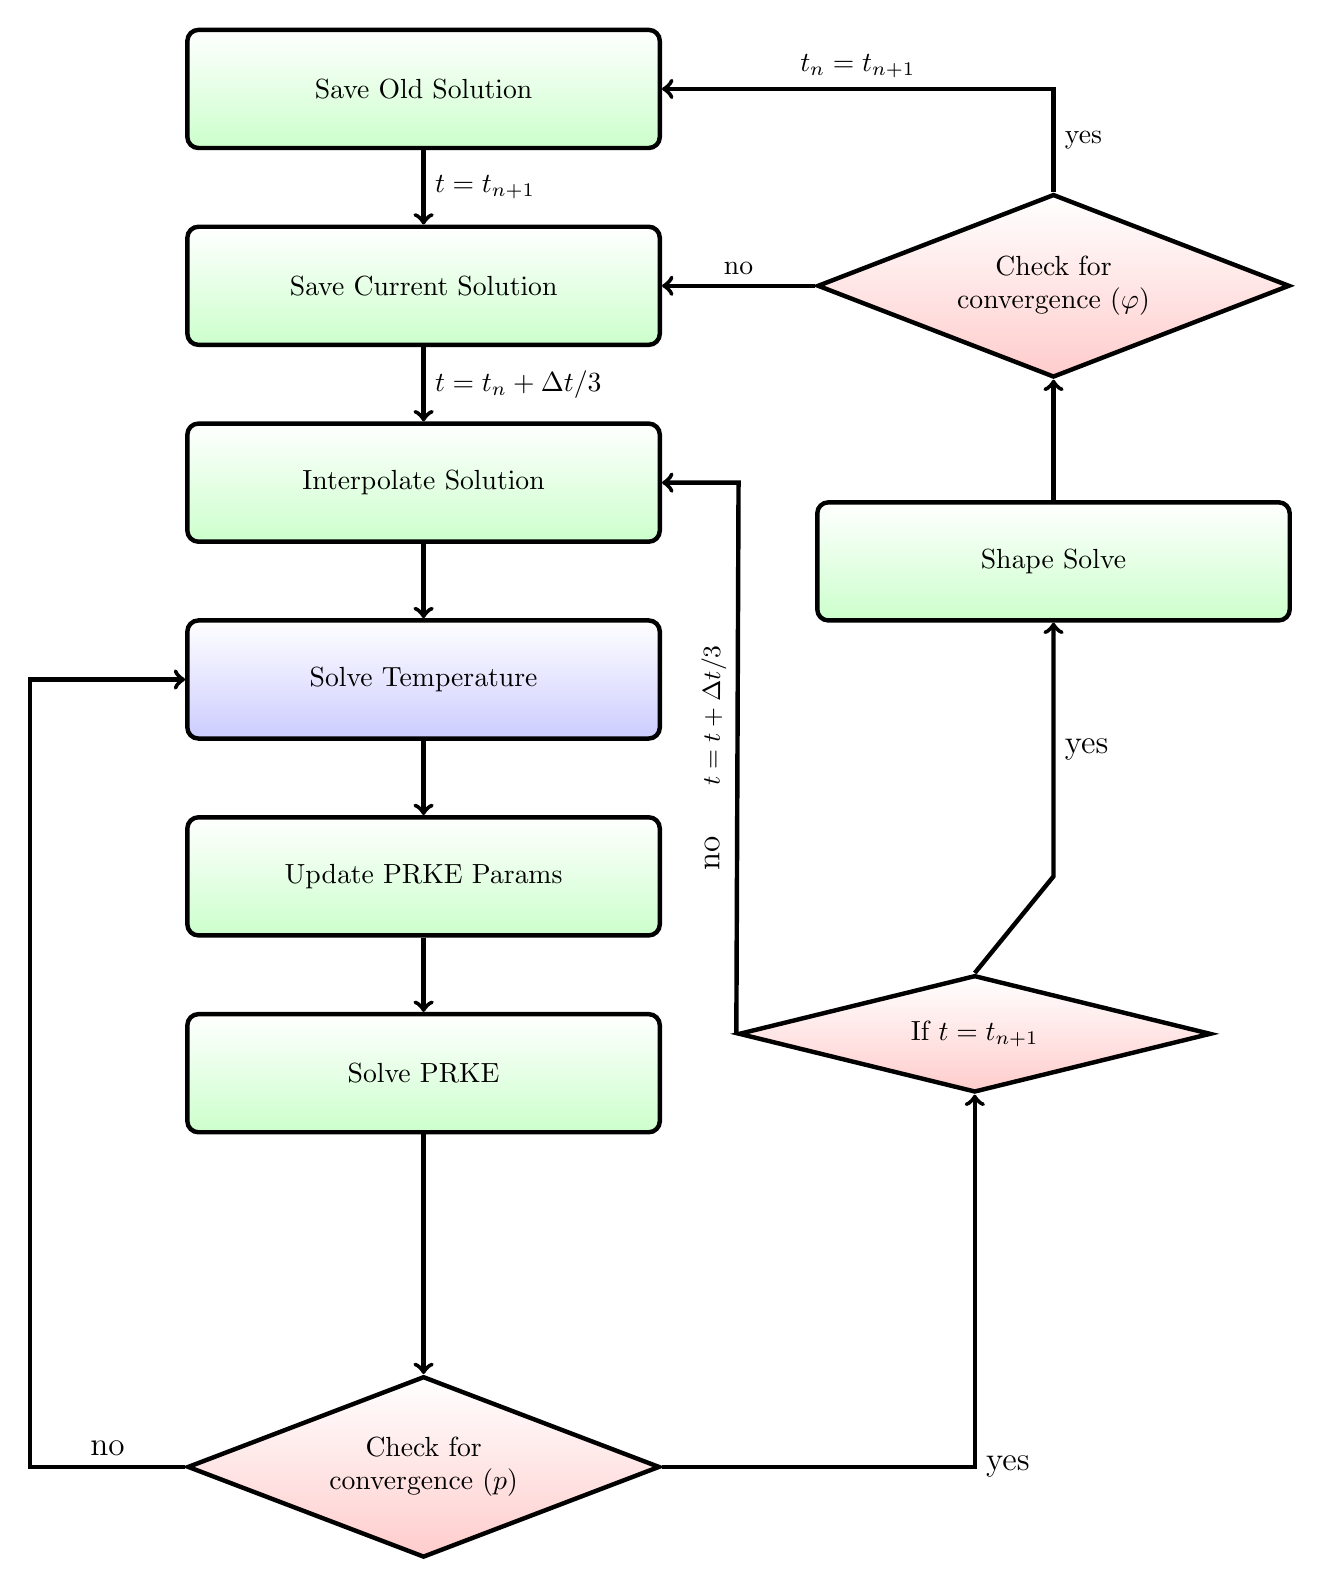
\begin{tikzpicture}[every node/.style = {font=\normalsize}]

\node[greenblock](p1) at (0,0) {Save Old Solution};
\node[greenblock](p2) at (0,-2.5) {Save Current Solution};
\node[greenblock](p3) at (0,-5) {Interpolate Solution};
\node[blueblock](p4) at (0,-7.5) {Solve Temperature};
\node[greenblock] (p5) at (0,-10) {Update PRKE Params};
\node[greenblock] (p6) at (0,-12.5) {Solve PRKE};
\node[reddiamond] (check1) at (0,-17.5) {Check for \\ convergence ($p$)};
\node[reddiamond] (check2) at (7,-12) {If $t=t_{n+1}$};
\node[greenblock] (p7) at (8,-6) {Shape Solve};
\node[reddiamond] (check3) at (8,-2.5) {Check for \\ convergence ($\varphi$)};
%\node [above =0.1mm of p1] {\large{IQS Solve:}};
%\node [above =0.1mm of p5] {\large{Multi-physics:}};

%\tikzback{p1}{p1}{p4}{p4}{bk1}
%\tikzback{p5}{p5}{p5}{p5}{bk2}

\draw[->,ultra thick](p1.south) -- node[right] {$t=t_{n+1}$}(p2.north);
\draw[->,ultra thick](p2.south) -- node[right] {$t=t_{n}+\Delta t/3$}(p3.north);
\draw[->,ultra thick](p3.south) -- (p4.north);
\draw [->,ultra thick] (p4.south)-- (p5.north);
\draw[->,ultra thick](p5.south) -- (p6.north);
\draw[->,ultra thick](p6.south) -- (check1.north);
\draw[->,ultra thick](check1.west) -- node[above,sloped] {\large{no}} (-5,-17.5) |-  (p4.west);
\draw[->,ultra thick](check1.east) -| node[right] {\large{yes}} (check2.south);
\draw[->,ultra thick](check2.west) -- node[above,sloped] {\large{no}\small \qq $t=t+\Delta t/3$} (4,-5) -- (p3.east);
\draw[->,ultra thick](check2.north) --  (8,-10) -- node[right] {\large{yes}} (p7.south);
\draw[->,ultra thick](p7.north) -- (check3.south);
\draw[->,ultra thick](check3.west) -- node[above] {no} (p2.east);
\draw[->,ultra thick](check3.north) -- node[right] {yes} (8,0) -- node[above] {$t_n=t_{n+1}$} (p1.east);

\end{tikzpicture}
\caption{Visualization of Picard iteration and temperature update process for regular IQS}
\label{fig:proc}
\end{figure}

\begin{figure}[!htpb]
\centering
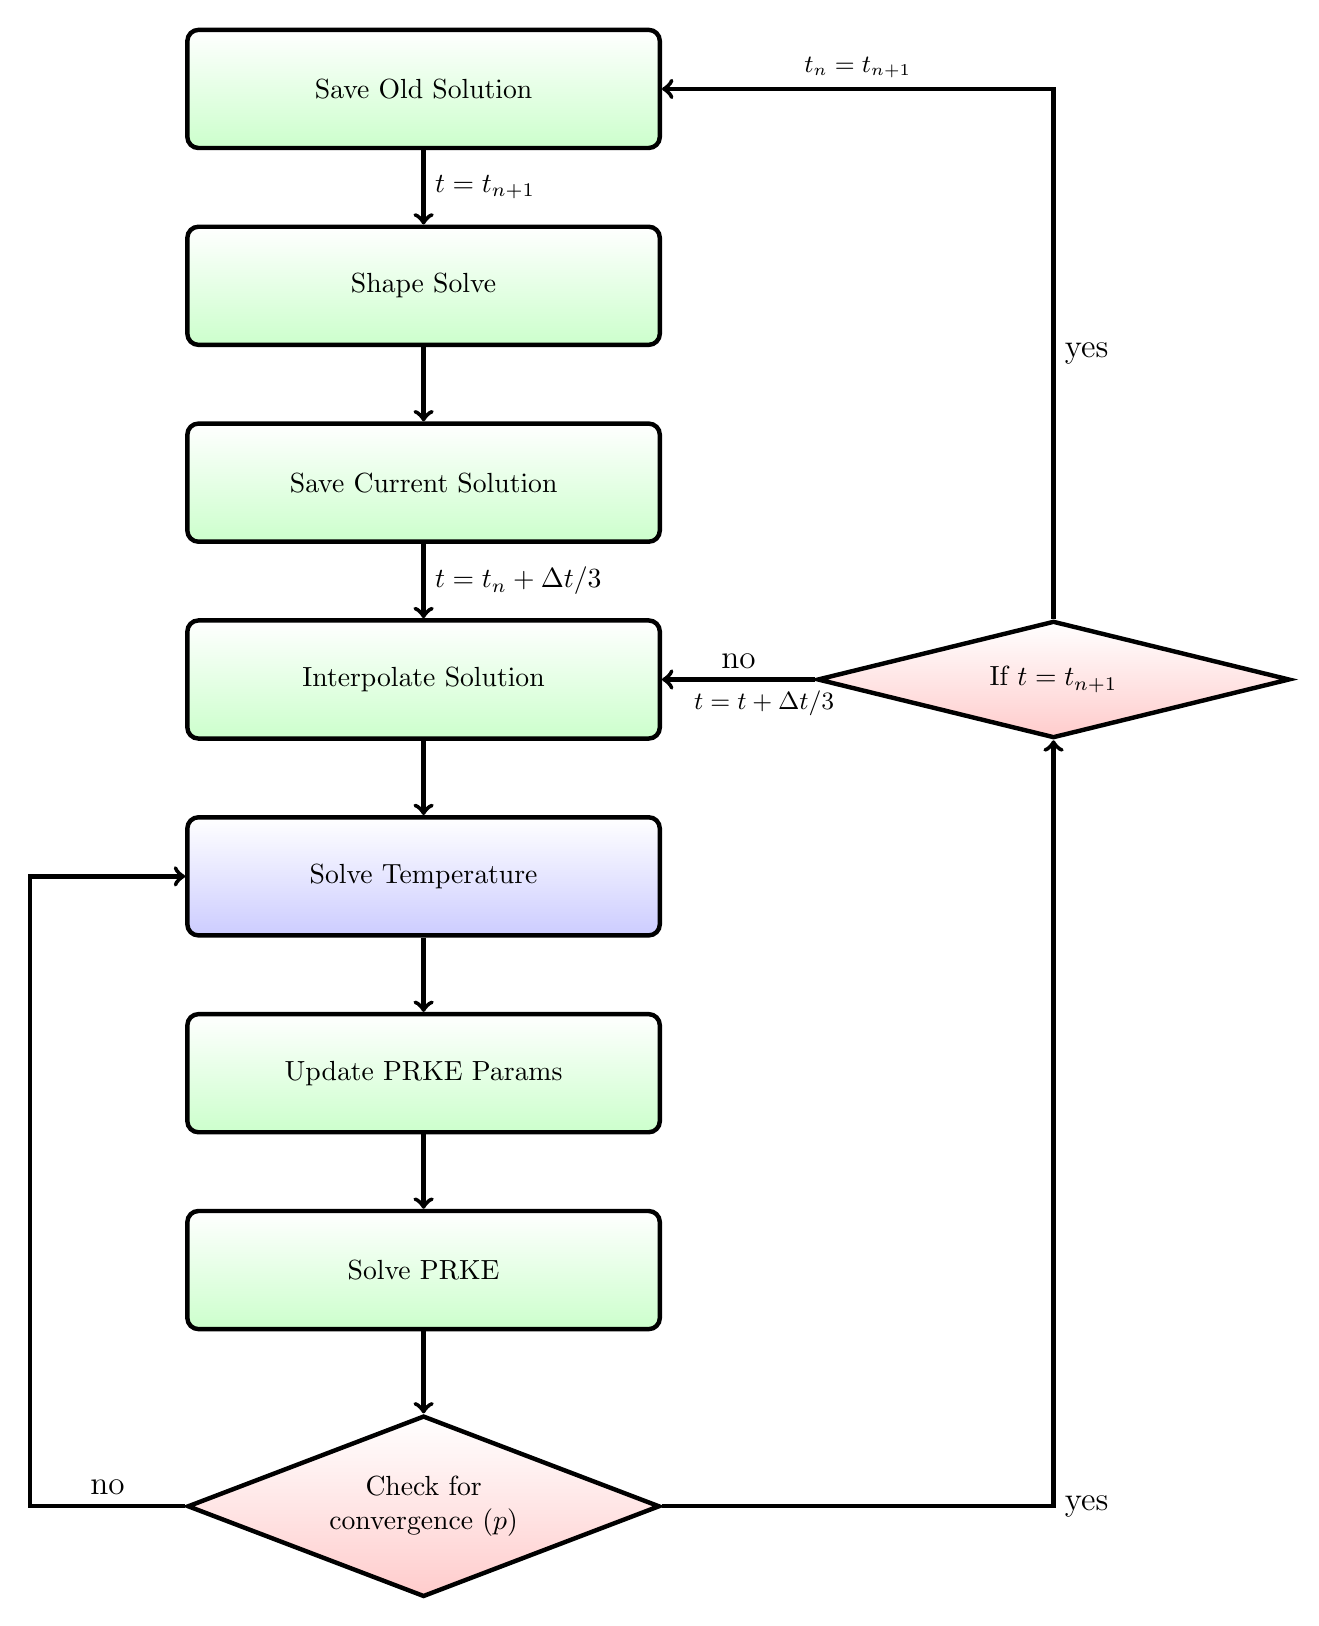
\begin{tikzpicture}[every node/.style = {font=\normalsize}]

\node[greenblock](p1) at (0,0) {Save Old Solution};
\node[greenblock](p2) at (0,-2.5) {Shape Solve};
\node[greenblock](p3) at (0,-5) {Save Current Solution};
\node[greenblock](p4) at (0,-7.5) {Interpolate Solution};
\node[blueblock](p5) at (0,-10) {Solve Temperature};
\node[greenblock] (p6) at (0,-12.5) {Update PRKE Params};
\node[greenblock] (p7) at (0,-15) {Solve PRKE};
\node[reddiamond] (check1) at (0,-18) {Check for \\ convergence ($p$)};
\node[reddiamond] (check2) at (8,-7.5) {If $t=t_{n+1}$};

%\tikzback{p1}{p1}{p4}{p4}{bk1}
%\tikzback{p5}{p5}{p5}{p5}{bk2}

\draw[->,ultra thick](p1.south) -- node[right] {$t=t_{n+1}$}(p2.north);
\draw[->,ultra thick](p2.south) -- (p3.north);
\draw[->,ultra thick](p3.south) -- node[right] {$t=t_{n}+\Delta t/3$} (p4.north);
\draw [->,ultra thick] (p4.south)-- (p5.north);
\draw[->,ultra thick](p5.south) -- (p6.north);
\draw[->,ultra thick](p6.south) -- (p7.north);
\draw[->,ultra thick](p7.south) -- (check1.north);
\draw[->,ultra thick](check1.west) -- node[above,sloped] {\large{no}} (-5,-18) |-  (p5.west);
\draw[->,ultra thick](check1.east) -| node[right] {\large{yes}} (check2.south);
\draw[->,ultra thick](check2.west) -- node[above,sloped] {\large{no}} node[below] {\small \qq $t=t+\Delta t/3$} (p4.east);
\draw[->,ultra thick](check2.north) -- node[right] {\large{yes}} (8,0) --  node[above] {\small $t_n=t_{n+1}$} (p1.east);

\end{tikzpicture}
\caption{Visualization of Picard iteration and temperature update process for IQS P-C}
\label{fig:procpc}
\end{figure}

\newpage
%%---------------------------------------------------------------------------%%
\section{\large Results}
%%---------------------------------------------------------------------------%%

This section describes the results of this implementation of temperature updates with the LRA benchmark.  Figure~\ref{fig:conv} shows the error convergence with 5 temperature updates per macro step.  It shows that with this amount of updates, IQS needs approximately a fourth of the time steps.  Figure~\ref{fig:mp} shows how various number of temperature updates affect the error with the same macro step size.  

\begin{figure}[H]
\centering
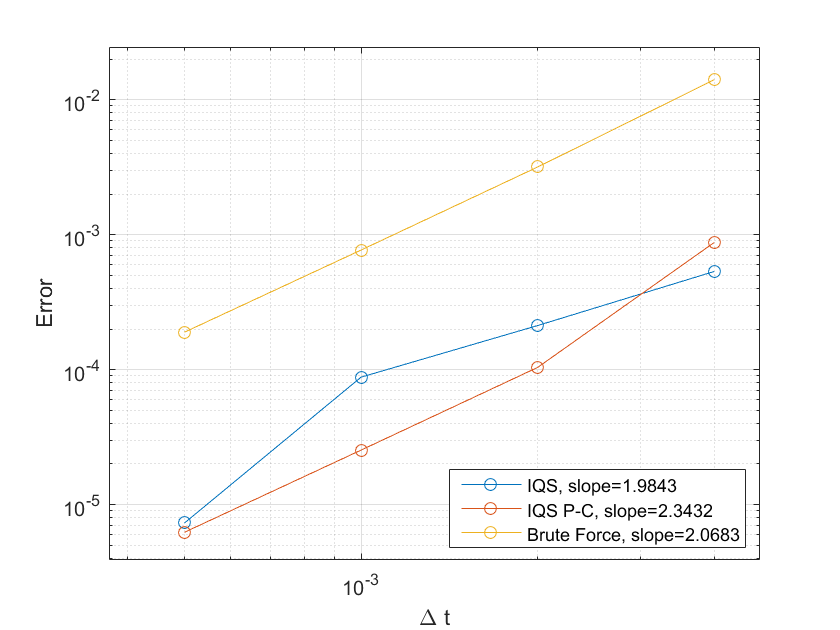
\includegraphics[height=4in]{mp_figs/lra_mp_convergence.png}
\caption{Error convergence plot with 5 temperature updates per macro step}
\label{fig:conv}
\end{figure}

\begin{figure}[H]
\centering
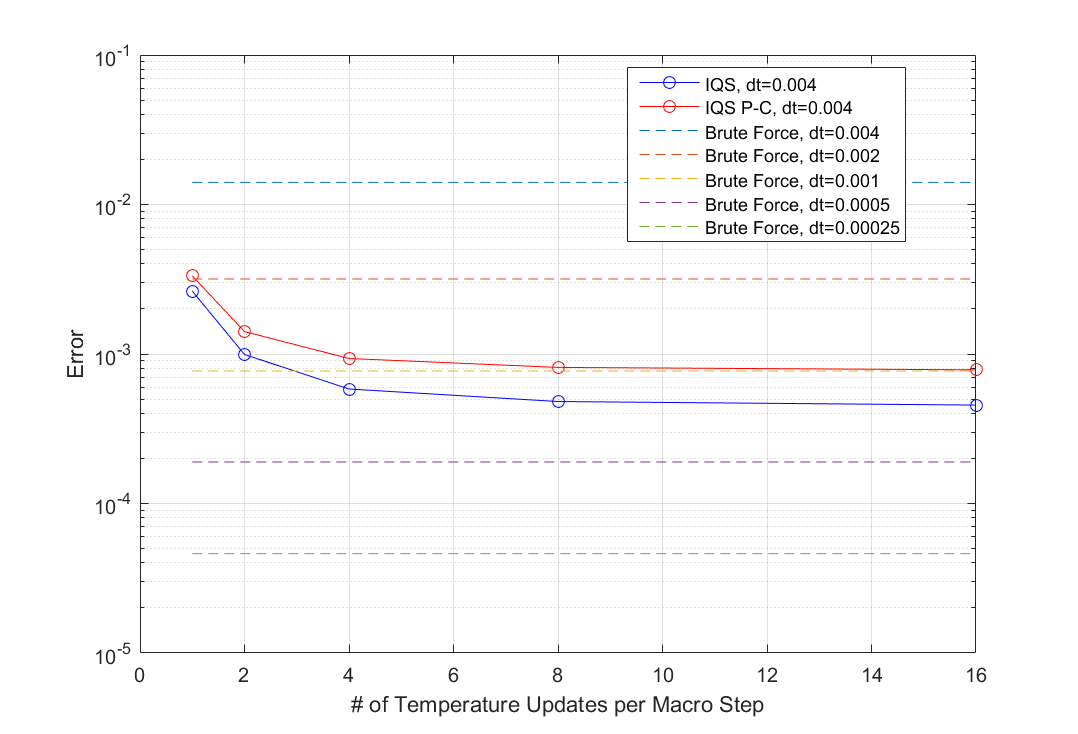
\includegraphics[height=4in]{mp_figs/lra_mp.png}
\caption{Error plot with various temperature updates per macro step}
\label{fig:mp}
\end{figure}

%%%%%%%%%%%%%%%%%%%%%%%%%%%%%%%%%%%%%%%%%%%%%%%%%%%%%%%%%%%%%%%%%%%%%%%%%%%%%%%%%%%%%%%%%%%%%%%%
%\newpage
%\closing
\end{document}
%%%%%%%%%%%%%%%%%%%%%%%%%%%%%%%%%%%%%%%%%%%%%%%%%%%%%%%%%%%%%%%%%%%%%%%%%%%%%%%%%%%%%%%%%%%%%%%%
